\documentclass{standalone}
\makeatletter\AtBeginDocument{\@buildstepset{1,2,3,4,5,6}}\makeatother
\usepackage{tikz}
\usetikzlibrary{intersections, calc}
\usepackage{hsbcommon}
\begin{document}
    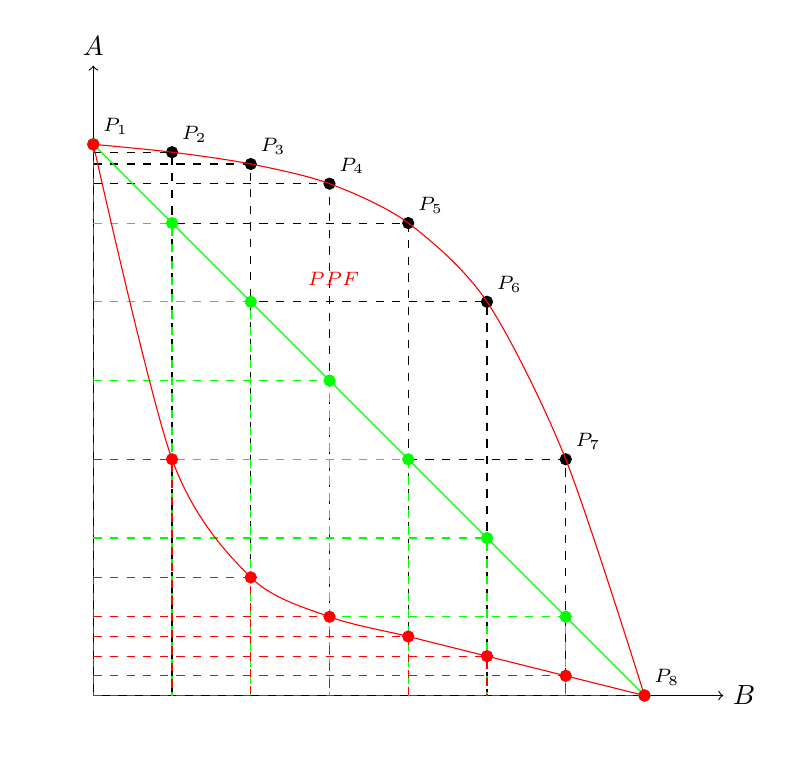
\begin{tikzpicture}
        \draw[->] (0,0) node[below] {\phantom{$X_i$}} -- (8,0) node[right]  {$B$};
        \draw[->] (0,0) node[left] {\phantom{$Y_mi$}} -- (0,8) node[above]  {$A$};

    %%%% increasing opportunity costs

    \coordinate (i0) at (0,7);
    \coordinate (i1) at (1,6.9);
    \coordinate (i2) at (2,6.75);
    \coordinate (i3) at (3,6.5);
    \coordinate (i4) at (4,6);
    \coordinate (i5) at (5,5);
    \coordinate (i6) at (6,3);
    \coordinate (i7) at (7,0);

    \ifstep{1}{
        \foreach [count=\i] \ii in {0,...,7}
            {
            \draw[dashed] (0, |- i\ii) -- (i\ii) -- (i\ii |-,0);
            \filldraw (i\ii) node[above right] {\scriptsize $P_\i$} circle (2pt);}
    }

    \ifstep{2}{    
        \draw[red] plot [smooth] coordinates {(i0) (i1) (i2) (i3) (i4)  (i5) (i6) (i7)} ;

        \node[red, below left=0.5cm] at (i4) {\scriptsize $PPF$};
    }    
    
    
    %%%% constant opportunity costs

    \begin{scope}[color=green]
        

    \coordinate (k0) at (0,7);
    \coordinate (k1) at (1,6);
    \coordinate (k2) at (2,5);
    \coordinate (k3) at (3,4);
    \coordinate (k4) at (4,3);
    \coordinate (k5) at (5,2);
    \coordinate (k6) at (6,1);
    \coordinate (k7) at (7,0);

    \ifstep{3}{
        \foreach [count=\i] \ii in {0,...,7}
            {
            \draw[dashed] (0, |- k\ii) -- (k\ii) -- (k\ii |-,0);
            \filldraw (k\ii) circle (2pt);}
    }

    \ifstep{4}{    
        \draw plot [smooth] coordinates {(k0) (k1) (k2) (k3) (k4) (k5) (k6) (k7)};
    }    
    \end{scope}

    %%%% inverted

    \ifstep{5}{
    
    \begin{scope}[color=red]
    
        \coordinate (l0) at (0,7);
        \coordinate (l1) at (1,3);
        \coordinate (l2) at (2,1.5);
        \coordinate (l3) at (3,1);
        \coordinate (l4) at (4,0.75);
        \coordinate (l5) at (5,0.5);
        \coordinate (l6) at (6,0.25);
        \coordinate (l7) at (7,0);
    
        \foreach [count=\i] \ii in {0,...,7}
            {
            \draw[dashed] (0, |- l\ii) -- (l\ii) -- (l\ii |-,0);
            \filldraw (l\ii)  circle (2pt);}

        \draw  plot [smooth] coordinates {(l0) (l1) (l2) (l3) (l4) (l5) (l6) (l7)};
    \end{scope}
    }
    

    \end{tikzpicture}
\end{document}
